\section{Build pipelines}
\label{sec:buildpipelines}

%% Graphic of build pipeline components
\begin{figure} % h-ere, t-op, b-ottom, p-age
    \centering
    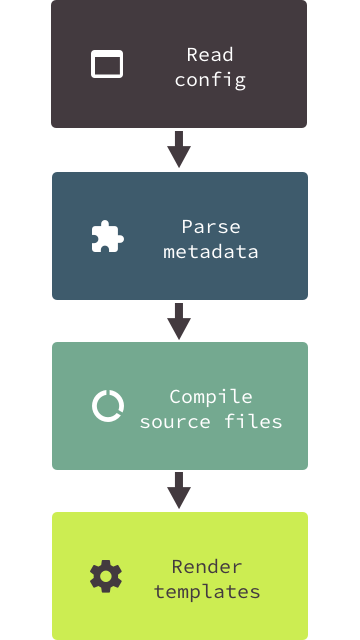
\includegraphics[width=0.333333\textwidth]{build_pipeline.png}
    \caption{A graphic showing the basic flow of a \emph{build pipeline}.\\
    At first, the configuration file is read and necessary modules invoked. Second, the global metadata, as well as metadata from within the content, is parsed and stored in the global configuration. Third, the content sources get compiled into basic \texttt{HTML} structures. Last, the compiled content gets rendered into predefined templates, to apply a common markup, which is used throughout the website and probably styled using \texttt{CSS}.}
    \label{fig:build-pipeline}
\end{figure}
%

A static site generator mostly consists of a \emph{build pipeline}, it handles the workflow needed for bringing the content in shape. This goes from setting the boundaries, determined in a configuration file, to finally compiling the content sources into a certain \texttt{HTML} structure and combining it with additional elements, included in template files (See Fig. \ref{fig:build-pipeline}).
